The adaptive study starts from 200 randomly chosen PyNite analyses and adds 200 per round up to 1{,}200, training a three-network ensemble (100 epochs) in every round; the whole study is repeated with two random seeds, and Fig.~\ref{fig:adaptive} shows the seed mean with the range of the two runs. Table~\ref{tab:adaptive} lists the errors at the final budget. Because these ensembles are smaller and trained on fewer frames for fewer epochs, their errors are higher than those of the main model in Table~\ref{tab:main}.

\begin{figure}[t]
\centering
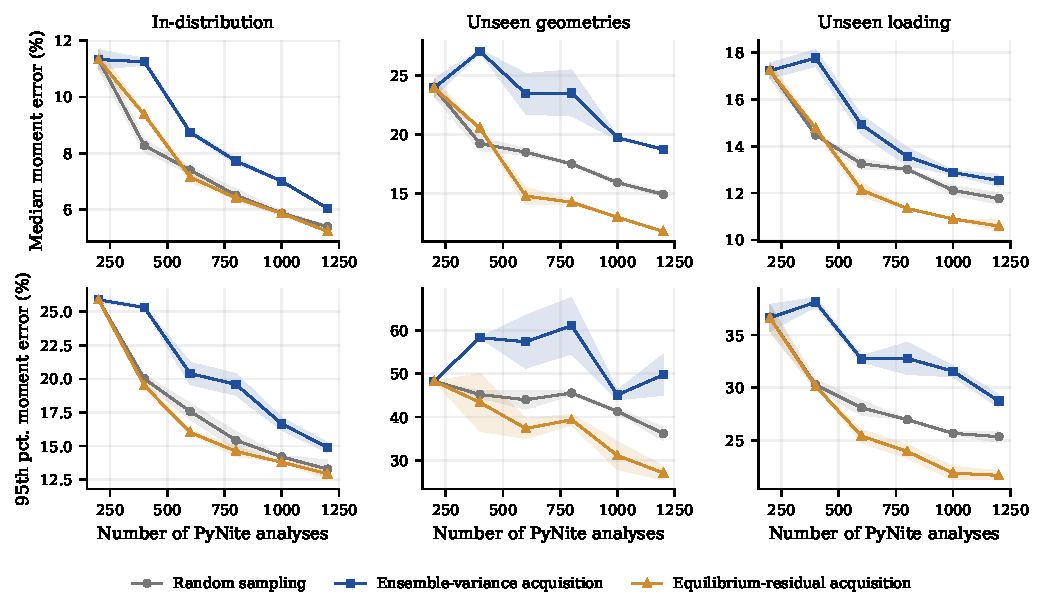
\includegraphics[width=\textwidth]{fig_adaptive.pdf}
\caption{Moment error (median, top; 95th percentile, bottom) versus the number of PyNite analyses used for training, for three acquisition rules. Lines: mean of two seeds; bands: range of the two seeds. Predictions include the variance-weighted projection.}\label{fig:adaptive}
\end{figure}

\begin{table}[t]
\centering
\caption{Errors (\%) after 1{,}200 PyNite analyses for each acquisition rule (mean of two seeds): median and 95th percentile of the moment error and median horizontal displacement error.}\label{tab:adaptive}
\scriptsize
\setlength{\tabcolsep}{3.5pt}
\begin{adjustbox}{max width=\textwidth}
\begin{tabular}{lrrrrrrrrr}
\toprule
& \multicolumn{3}{c}{In-distribution} & \multicolumn{3}{c}{Unseen geometries} & \multicolumn{3}{c}{Unseen loading}\\
\cmidrule(lr){2-4}\cmidrule(lr){5-7}\cmidrule(lr){8-10}
Acquisition & $e_M$ & $e_M$ (p95) & $e_{u_x}$ & $e_M$ & $e_M$ (p95) & $e_{u_x}$ & $e_M$ & $e_M$ (p95) & $e_{u_x}$\\
\midrule
\inputtable{tables/tab_adaptive.tex}
\bottomrule
\end{tabular}
\end{adjustbox}
\end{table}

Two findings stand out. First, selecting the frames with the largest ensemble variance is \emph{worse} than random sampling on all three test sets and for both seeds (median moment error 6.0\% vs.\ 5.4\% ID, 18.8\% vs.\ 14.9\% OOD-G at 1{,}200 analyses). Greedy top-$B$ selection by variance concentrates the budget on the most extreme corners of the design space, typically frames with very flexible members or unusual stiffness ratios, at the expense of coverage of the bulk of the distribution; a batch of 200 such frames is also highly redundant. Second, selecting the frames whose raw prediction is furthest from equilibrium is the best of the three rules for the member forces on every test set: at 1{,}200 analyses the median moment error is 5.2\% (random 5.4\%) on ID frames, 11.8\% (14.9\%) on unseen geometries and 10.6\% (11.8\%) on unseen loading, and the 95th percentile on unseen geometries falls from 36.2\% to 27.1\%. On unseen geometries the equilibrium-residual rule reaches the final error of random sampling after 600 analyses, i.e.\ with half the FE budget, and on unseen loading after 800. The gain is specific to forces: the displacement errors are similar to or slightly larger than with random sampling (Table~\ref{tab:adaptive}), which is expected, since the residual measures the admissibility of the forces only. With two seeds, the differences between the equilibrium-residual rule and random sampling on the ID set are within the seed-to-seed spread, whereas those on the unseen sets are consistent across both seeds.
